\documentclass{amsart}
\usepackage{graphicx}
\usepackage[RGB]{xcolor}
\usepackage{tikz}

% \colorsquare{#1: color}{#2 x-coordinate}{#3: y-coordinate}
% the bottom left coordinate is (1,1), and the topright of an nxn square is (n,n)
\newcommand{\colorsquare}[3]{
\coordinate (pos) at (#2-1,#3-1);
\filldraw[color=#1] (pos)--++(1,0)--++(0,1)--++(-1,0)--cycle;
}

% \numbersquare{#1: int}{#2: x-coordinate}{#3: y-coordinate}
% uses the same coordinate scheme as \colorsquare
\newcommand{\numbersquare}[3]{\draw(#2-.5, #3-.5) node {\LARGE $\mathsf{#1}$};}

\newcommand{\drawthick}{\draw[line width=1.75pt]}

\definecolor{I}{RGB}{238,170,169}
\definecolor{F}{RGB}{220,187,153}
\definecolor{L}{RGB}{204,204,136}
\definecolor{P}{RGB}{186,221,153}
\definecolor{N}{RGB}{169,238,170}
\definecolor{T}{RGB}{153,221,187}
\definecolor{U}{RGB}{136,204,204}
\definecolor{V}{RGB}{153,187,221}
\definecolor{W}{RGB}{170,170,238}
\definecolor{X}{RGB}{186,153,221}
\definecolor{Y}{RGB}{204,136,204}
\definecolor{Z}{RGB}{221,153,186}

% \drawgrid{#1: int}
% draws an #1x#1 grid with thick lines around the border
\newcommand{\drawgriddotted}[1]{
    \foreach \x in {0,...,#1}{
    \draw[densely dotted] (\x,#1)--(\x,0);
    }
    \foreach \y in {0,...,#1}{
      \draw[densely dotted] (0,\y)--(#1,\y);
    }
   \drawthick (0,0)--(0,#1)--(#1,#1)--(#1,0)--cycle;
}

\newcommand{\drawgridthin}[1]{
    \foreach \x in {0,...,#1}{
    \draw[very thin] (\x,#1)--(\x,0);
    }
    \foreach \y in {0,...,#1}{
      \draw[very thin] (0,\y)--(#1,\y);
    }
   \drawthick (0,0)--(0,#1)--(#1,#1)--(#1,0)--cycle;
}
    
\begin{document}
\resizebox{30pc}{!}{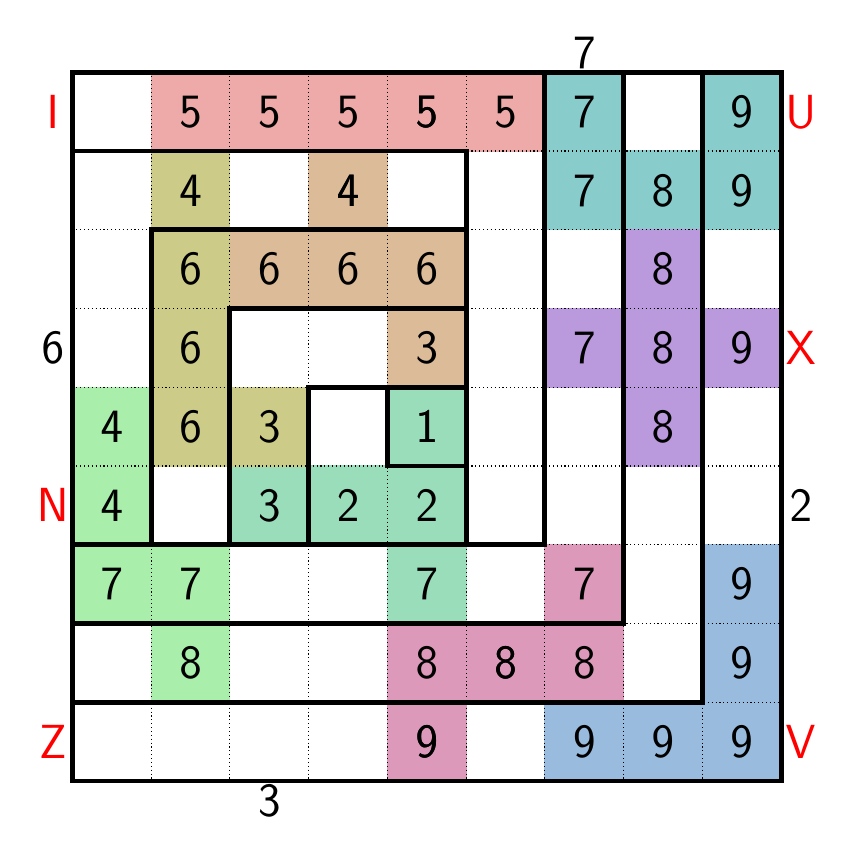
\begin{tikzpicture}
\colorsquare{I}{6}{9}\colorsquare{I}{2}{9}\colorsquare{I}{3}{9}\colorsquare{I}{4}{9}\colorsquare{I}{5}{9}
\colorsquare{U}{8}{8}\colorsquare{U}{7}{8}\colorsquare{U}{9}{9}\colorsquare{U}{7}{9}\colorsquare{U}{9}{8}
\colorsquare{X}{8}{5}\colorsquare{X}{7}{6}\colorsquare{X}{8}{6}\colorsquare{X}{8}{7}\colorsquare{X}{9}{6}
\colorsquare{Z}{6}{2}\colorsquare{Z}{5}{2}\colorsquare{Z}{5}{1}\colorsquare{Z}{7}{3}\colorsquare{Z}{7}{2}
\colorsquare{V}{7}{1}\colorsquare{V}{8}{1}\colorsquare{V}{9}{3}\colorsquare{V}{9}{2}\colorsquare{V}{9}{1}
\colorsquare{F}{3}{7}\colorsquare{F}{4}{7}\colorsquare{F}{5}{6}\colorsquare{F}{4}{8}\colorsquare{F}{5}{7}
\colorsquare{T}{4}{4}\colorsquare{T}{3}{4}\colorsquare{T}{5}{5}\colorsquare{T}{5}{3}\colorsquare{T}{5}{4}
\colorsquare{N}{2}{2}\colorsquare{N}{1}{3}\colorsquare{N}{1}{4}\colorsquare{N}{1}{5}\colorsquare{N}{2}{3}
\colorsquare{L}{3}{5}\colorsquare{L}{2}{7}\colorsquare{L}{2}{6}\colorsquare{L}{2}{5}\colorsquare{L}{2}{8}
\drawthick (8,0)--++(-8,0)--++(0,1)--++(8,0)--++(0,8)--++(1,0)--++(0,-9)--cycle;
    \drawthick (7,1)--++(-7,0)--++(0,1)--++(7,0)--++(0,7)--++(1,0)--++(0,-8)--cycle;
    \drawthick (6,2)--++(-6,0)--++(0,1)--++(6,0)--++(0,6)--++(1,0)--++(0,-7)--cycle;
    \drawthick (5,8)--++(-5,0)--++(0,1)--++(6,0)--++(0,-6)--++(-1,0)--cycle;
    \drawthick (0,7)--++(0,1)--++(5,0)--++(0,-1)--++(-4,0)--++(0,-4)--++(-1,0)--cycle;
    \drawthick (1,6)--++(0,1)--++(4,0)--++(0,-1)--++(-3,0)--++(0,-3)--++(-1,0)--cycle;
    \drawthick (2,5)--++(0,1)--++(3,0)--++(0,-1)--++(-2,0)--++(0,-2)--++(-1,0)--cycle;
    \drawthick (3,3)--++(0,2)--++(1,0)--++(0,-1)--++(1,0)--++(0,-1)--cycle;\drawgriddotted{9}\numbersquare{1}{5}{5}\numbersquare{9}{5}{1}\numbersquare{8}{6}{2}\numbersquare{4}{4}{8}\numbersquare{5}{5}{9}\numbersquare{3}{3.0}{0.25}\numbersquare{2}{9.75}{4.0}\numbersquare{6}{0.25}{6.0}\numbersquare{7}{7.0}{9.75}\numbersquare{\textcolor{red}{I}}{0.25}{9.0}\numbersquare{\textcolor{red}{N}}{0.25}{4.0}\numbersquare{\textcolor{red}{Z}}{0.25}{1.0}\numbersquare{\textcolor{red}{V}}{9.75}{1.0}\numbersquare{\textcolor{red}{X}}{9.75}{6.0}\numbersquare{\textcolor{red}{U}}{9.75}{9.0}\numbersquare{5}{6}{9}\numbersquare{5}{2}{9}\numbersquare{5}{3}{9}\numbersquare{5}{4}{9}\numbersquare{5}{5}{9}\numbersquare{8}{8}{8}\numbersquare{7}{7}{8}\numbersquare{9}{9}{9}\numbersquare{7}{7}{9}\numbersquare{9}{9}{8}\numbersquare{8}{8}{5}\numbersquare{7}{7}{6}\numbersquare{8}{8}{6}\numbersquare{8}{8}{7}\numbersquare{9}{9}{6}\numbersquare{8}{6}{2}\numbersquare{8}{5}{2}\numbersquare{9}{5}{1}\numbersquare{7}{7}{3}\numbersquare{8}{7}{2}\numbersquare{9}{7}{1}\numbersquare{9}{8}{1}\numbersquare{9}{9}{3}\numbersquare{9}{9}{2}\numbersquare{9}{9}{1}\numbersquare{6}{3}{7}\numbersquare{6}{4}{7}\numbersquare{3}{5}{6}\numbersquare{4}{4}{8}\numbersquare{6}{5}{7}\numbersquare{2}{4}{4}\numbersquare{3}{3}{4}\numbersquare{1}{5}{5}\numbersquare{7}{5}{3}\numbersquare{2}{5}{4}\numbersquare{8}{2}{2}\numbersquare{7}{1}{3}\numbersquare{4}{1}{4}\numbersquare{4}{1}{5}\numbersquare{7}{2}{3}\numbersquare{3}{3}{5}\numbersquare{6}{2}{7}\numbersquare{6}{2}{6}\numbersquare{6}{2}{5}\numbersquare{4}{2}{8}\end{tikzpicture}}
\vspace{1pc}

\noindent\Large{\tt The product of the areas of the connected unfilled squares is 1620}
\end{document}